
\begin{figure}[t!]
    \centering
    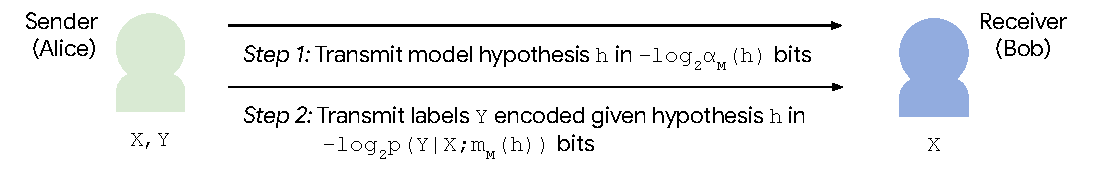
\includegraphics[width=0.85\columnwidth,keepaspectratio]{figures/two_part_code_pdf.pdf}
    \caption{\textbf{Two-part code.} One way to formalize the MDL principle is with a two-part code. %
    Assume Alice and Bob agree on a two-part code $M$ and each are given inputs $X$. Alice then finds the hypothesis (e.g., model parameters) that enables sending Bob the labels $Y$ in the fewest total bits, balancing the complexity of the model with how well it fits the data. One key challenge we address is that the minimum codelength is dependent on the potentially arbitrary choice of prior $\alpha_M(h)$. %
    }
    \label{fig:two_part_code}
\end{figure}
